\documentclass[crop,tikz]{standalone}

\usepackage[utf8]{inputenc}
\usepackage{fouriernc}
\usepackage[T1]{fontenc}
\usepackage{bm}
\usepackage{amsmath}
\usepackage{trfsigns}
\usepackage{xcolor}
\usetikzlibrary{arrows.meta}

%matplotlib colors:
\definecolor{C0}{HTML}{1f77b4}
\definecolor{C1}{HTML}{ff7f0e}
\definecolor{C2}{HTML}{2ca02c}
\definecolor{C3}{HTML}{d62728}
\definecolor{C4}{HTML}{9467bd}
\definecolor{C5}{HTML}{8c564b}
\definecolor{C6}{HTML}{e377c2}
\definecolor{C7}{HTML}{7f7f7f}
\definecolor{C8}{HTML}{bcbd22}
\definecolor{C9}{HTML}{17becf}

\begin{document}
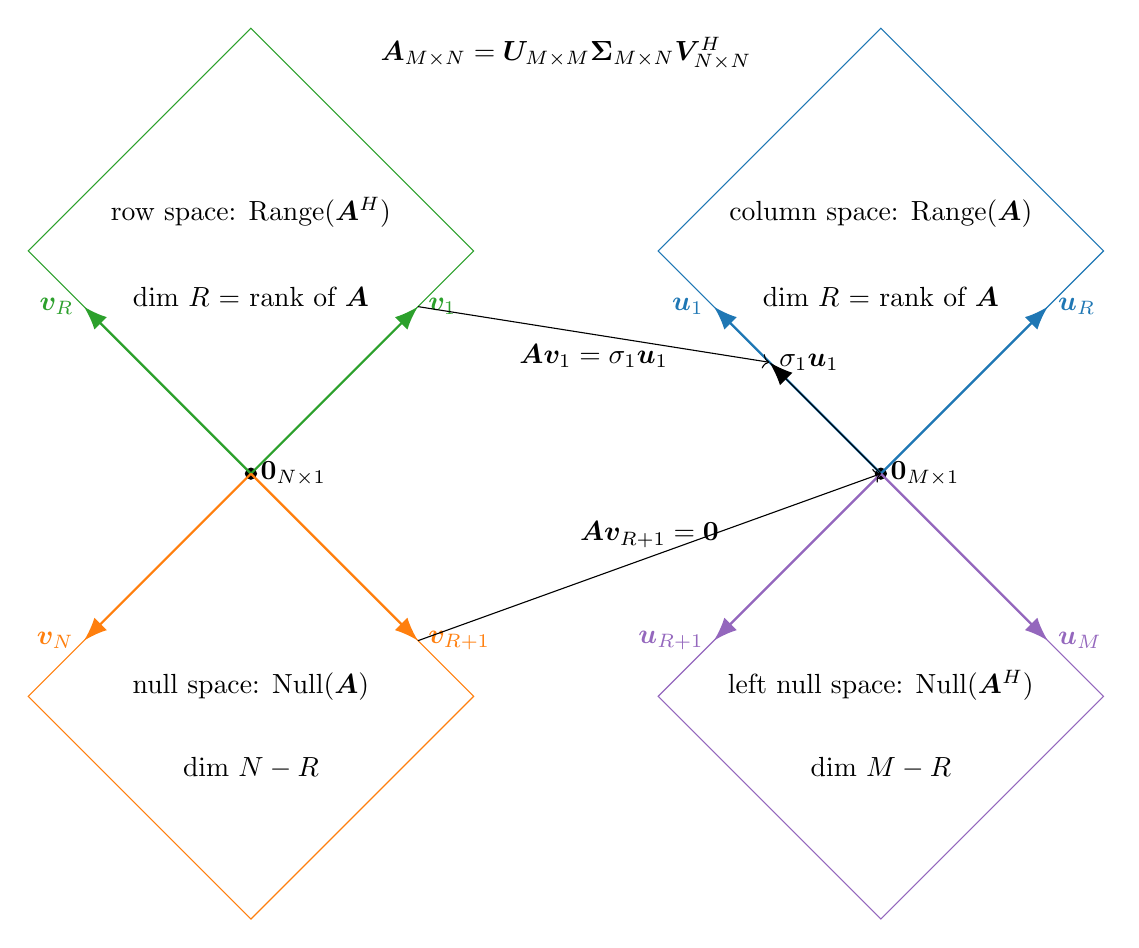
\begin{tikzpicture}

\coordinate (u_space) at (+4,0);
\coordinate (v_space) at (-4,0);
\def\lengthrect{4};
\def\lengthvec{3};

\path (0,0) +(90:\lengthvec+2) coordinate (G);
\draw (G) node[above]{$\bm{A}_{M \times N} = \bm{U}_{M \times M} \bm{\Sigma}_{M \times N} \bm{V}_{N \times N}^H$};

\draw[draw=black, rotate around={45:(u_space)}, C0] (u_space) rectangle ++(\lengthrect,\lengthrect);
\draw[draw=black, rotate around={225:(u_space)}, C4] (u_space) rectangle ++(\lengthrect,\lengthrect);

\draw[draw=black, rotate around={45:(v_space)}, C2] (v_space) rectangle ++(\lengthrect,\lengthrect);
\draw[draw=black, rotate around={225:(v_space)}, C1] (v_space) rectangle ++(\lengthrect,\lengthrect);

%zero vectors
\draw[fill] (u_space) circle (2pt) node[right]{$\bm{0}_{M \times 1}$};
\draw[fill] (v_space) circle (2pt) node[right]{$\bm{0}_{N \times 1}$};

% U space stuff:
\path (u_space) +(135:\lengthvec) coordinate (u1);
\draw[-{Latex[length=3mm]}, C0, thick] (u_space) -- (u1) node[left]{$\bm{u}_1$};

\path (u_space) +(45:\lengthvec) coordinate (ur);
\draw[-{Latex[length=3mm]}, C0, thick] (u_space) -- (ur) node[right]{$\bm{u}_R$};

\path (u_space) +(225:\lengthvec) coordinate (ur1);
\draw[-{Latex[length=3mm]}, C4, thick] (u_space) -- (ur1) node[left]{$\bm{u}_{R+1}$};

\path (u_space) +(315:\lengthvec) coordinate (um);
\draw[-{Latex[length=3mm]}, C4, thick] (u_space) -- (um) node[right]{$\bm{u}_{M}$};

\path (u_space) +(90:\lengthvec) coordinate (col_space);
\draw (col_space) node[above]{column space: $\text{Range}(\bm{A})$};

\path (u_space) +(90:\lengthvec-1) coordinate (col_space_dim);
\draw (col_space_dim) node[above]{dim $R$ = rank of $\bm{A}$};

\path (u_space) +(270:\lengthvec) coordinate (left_null_space);
\draw (left_null_space) node[above]{left null space: $\text{Null}(\bm{A}^H)$};

\path (u_space) +(270:\lengthvec+1) coordinate (left_null_space_dim);
\draw (left_null_space_dim) node[above]{dim $M-R$};

% V space stuff:
\path (v_space) +(45:\lengthvec) coordinate (v1);
\draw[-{Latex[length=3mm]}, C2, thick] (v_space) -- (v1) node[right]{$\bm{v}_1$};

\path (v_space) +(135:\lengthvec) coordinate (vr);
\draw[-{Latex[length=3mm]}, C2, thick] (v_space) -- (vr) node[left]{$\bm{v}_R$};

\path (v_space) +(315:\lengthvec) coordinate (vr1);
\draw[-{Latex[length=3mm]}, C1, thick] (v_space) -- (vr1) node[right]{$\bm{v}_{R+1}$};

\path (v_space) +(225:\lengthvec) coordinate (vn);
\draw[-{Latex[length=3mm]}, C1, thick] (v_space) -- (vn) node[left]{$\bm{v}_{N}$};

\path (v_space) +(90:\lengthvec) coordinate (row_space);
\draw (row_space) node[above]{row space: $\text{Range}(\bm{A}^H)$};

\path (v_space) +(90:\lengthvec-1) coordinate (row_space_dim);
\draw (row_space_dim) node[above]{dim $R$ = rank of $\bm{A}$};

\path (v_space) +(270:\lengthvec) coordinate (null_space);
\draw (null_space) node[above]{null space: $\text{Null}(\bm{A})$};

\path (v_space) +(270:\lengthvec+1) coordinate (null_space_dim);
\draw (null_space_dim) node[above]{dim $N-R$};

% row to column
\path (u_space) +(135:\lengthvec-1) coordinate (u1s);
\draw[-{Latex[length=3mm]}] (u_space) -- (u1s) node[right]{$\sigma_1 \bm{u}_1$};
\draw[->] (v1) -- node[below]{$\bm{A} \bm{v}_1=\sigma_1 \bm{u}_1$}(u1s);

% null to zero vec
\draw[->] (vr1) -- node[above]{$\bm{A} \bm{v}_{R+1}=\bm{0}$}(u_space);

\end{tikzpicture}
\end{document}
